\documentclass[]{article}
\usepackage[left=2.5cm,right=2.5cm,top=2.0cm,bottom=2.5cm]{geometry}
\usepackage{graphicx}
\usepackage{hyperref}
\graphicspath{.}
\title{System Call Proxy Protocol}
\begin{document}
\maketitle

\section{Introduction}

This document describes a distributed dataplane to support clustered
operating system functions. For no strong reason we have selected
triples, or entity-attribte-value(EAV) assertions as the foundation.
Arbitrary length tuples with schema, basically relational tables is another
suitable substrate, as is a simple nested hierarchy. 

We put a little structure around our triples and then address some of the
issues around distributed evaluation of programs that operate on this
EAV graph. 

\section{Triples Model}
Triples came out of the semantic web, in a specification called RDF,
where unfrotuantely the mapping between XML and RDF was left
undefined (\href{https://en.wikipedia.org/wiki/Resource_Description_Framework}).
Objects in the system are given globally unique
identifiers. Each of these objects has a set of properties described
by the attribute field, and each attribute for an entity has exactly
one value. So we can view EAVs as really just a property list or
hashmap.

Since the value can be another entity, triples can also be used to
form a graph of entities with labelled edges. When developing schema
for this system (for some reason we use the word ontology), its quite
common for the attributes themselves to be objects, although this
isn't a usage we will pursue.

The objects of interest in our system are things like:
\begin{itemize}
   \item machines
   \item processes
   \item users
   \item files
\end{itemize}

It shouldn't be contentious that we can use this graph to model
operating system state, in particular the posix-esque semantics of
linux syscalls. If not, hopefully the following details will paint a
better picture.

\subsection{Entities}
Entities are the objects of our system, and to facilitate distribute
evaluation we will also use them as addresses for purposes of
routing. We also need to construct them in such a way that they can
efficiently generated, and that we can never have two objects anywhere
in the world with the same name.

There are probably too many dependencies on the ultimate distribution
methodology to make an authoratative design, but this can serve as
an illustrative example:\\
\vspace{0.2in}
\begin{center}
  \includegraphics[scale=0.8]{entity.pdf}
\end{center}  

\subsection{Attributes}
In many triple setups, the attributes are entities themselves. This allows
attribute metadata such as kind of modifier, historical information, references
into specifications, etc. At the other end of the spectrum attributes are
selected from a small set of predefined integers. For the initial system we propose a middle
ground, that attributes be freeform strings. In order to bring some modicum of
standardization and control to the layout of objects, we introduce a simple
schema definition to publish known keys and support validation. 

\subsection{Values}

\section{Schema}

\section{Commands}

\subsection{set(entity, attribute, value)}
\subsection{get(entity, attribute) -> value}
\subsection{copy(dest, source, length)}
Copies {\em length} bytes from the {\em source} bytestring to the {\em dest}. It
is an error if both the referred objects are not byte strings. For convenience if
the destination is an (entity, attribute) pair which current is unbound, then
the binding is created and set to the bytestring specified by the source address.


\subsection{Addresses}
The {\em source} and {\em dest} parameters are compound addresses. Addresses refer
to byte ranges in values.
\begin{description}
  \item {value(e, a)}
  \item {offset(A, count)}
  \item {region\_id(A, count)}    
\end{description}    

\section{Program Blocks}
Collections of commands are grouped together into {\em blocks}.



\section{Concurrency}
The

The current implementation does not provide any global isolation or
serializability for the execution of blocks. If services are provided on top of
a system like Linux, then its very difficult to introduce these concepts because
the underlying facilites aren't 2-phase - they cant in any way promise to commit.

\section{Security}
There is a nice design where blocks are signed by principals, and
contain signed statements of delegated authority. A user might start a
process and sign a statement including the processes new public key
and a set of grants in EAV space.

This setup directly contradicts the idea that programs can be rewritten to
effect evaluation policy. Most of the value of signed delegation comes from its
end-to-end to property. The provider of a service doesn't have to trust the network,
just the principal for which it has it own chain of trust. Re-signing subrequests
puts in back in a position where we need to trust everyone.


    
\section{Errors}
\end{document}
